\documentclass[9pt]{beamer}

% Beamer style
%\usetheme[secheader]{Madrid}
% \usetheme{CambridgeUS}
\useoutertheme{infolines}
\usecolortheme[rgb={0.65,0.15,0.25}]{structure}
% \usefonttheme[onlymath]{serif}
\beamertemplatenavigationsymbolsempty
%\AtBeginSubsection

% Packages
%\usepackage[french]{babel}
\usepackage[latin1]{inputenc}
\usepackage{color}
\usepackage{xspace}
\usepackage{dsfont, stmaryrd}
\usepackage{amsmath, amsfonts, amssymb, stmaryrd}
\usepackage{epsfig}
\usepackage{tikz}
\usepackage{url}
% \usepackage{ulem}
\usepackage{/home/robin/LATEX/Biblio/astats}
%\usepackage[all]{xy}
\usepackage{graphicx}
\usepackage{xspace}

\input{/home/robin/RECHERCHE/EXPOSES/LATEX/Commands}
\newcommand{\CTSBM}{{\sl ct}-SBM\xspace}
\newcommand{\DTSBM}{{\sl dt}-SBM\xspace}

% Directory
\newcommand{\fignet}{/home/robin/Bureau/RECHERCHE/RESEAUX/EXPOSES/FIGURES}
\newcommand{\figchp}{/home/robin/Bureau/RECHERCHE/RUPTURES/EXPOSES/FIGURES}
% \newcommand{\figfig}{../figs}
\newcommand{\figCMR}{/home/robin/Bureau/RECHERCHE/ECOLOGIE/CountPCA/sparsepca/Article/Network_JCGS/trunk/figs}
\newcommand{\figDoR}{/home/robin/Bureau/RECHERCHE/BAYES/VBEM-IS/VBEM-IS.git/Data/Tree/Fig}


%====================================================================
%====================================================================

%====================================================================
%====================================================================
\begin{document}
%====================================================================
%====================================================================

%====================================================================
\section*{Ecological network inference}
\frame{\frametitle{Typical situation}

\paragraph{Barents fish \refer{FNA06}:} $n = 89$ sites, $m = 30$ species, $d = 4$ covariates

\bigskip \pause
\begin{tabular}{c|c|c}
  \onslide+<2->{\paragraph{Abundances $Y$:} $n \times m$}
  & 
  \onslide+<3->{\paragraph{Covariates $X$:} $n \times d$}
  & 
  \onslide+<4>{\paragraph{Network $G$:} $m \times m$ }
  \\
  \hspace{-.02\textwidth} 
  \begin{tabular}{p{.3\textwidth}}
    \onslide+<2->{\begin{tabular}{rrr}
      {\sl Hi.pl} & {\sl An.lu} & {\sl Me.ae} 
      \footnote{{\sl Hi.pl}: Long rough dab, {\sl An.lu}: Atlantic wolffish, {\sl Me.ae}: Haddock} \\ 
%       Dab & Wolffish & Haddock \\ 
      \hline
      31  &   0  & 108 \\
       4  &   0  & 110 \\
      27  &   0  & 788 \\
      13  &   0  & 295 \\
      23  &   0  &  13 \\
      20  &   0  &  97 \\
      \vdots & \vdots & \vdots 
    \end{tabular}} 
  \end{tabular}
  & 
  \begin{tabular}{p{.3\textwidth}}
    \onslide+<3->{\begin{tabular}{rrr}
      Lat. & Long. & Depth \\ \hline
      71.10 & 22.43 & 349 \\
      71.32 & 23.68 & 382 \\
      71.60 & 24.90 & 294 \\
      71.27 & 25.88 & 304 \\
      71.52 & 28.12 & 384 \\
      71.48 & 29.10 & 344 \\
      \vdots & \vdots & \vdots 
    \end{tabular}} 
  \end{tabular}
  & 
  \hspace{-.02\textwidth} \pause
  \begin{tabular}{p{.3\textwidth}}
    \onslide+<4>{\hspace{-.1\textwidth} 
      \begin{tabular}{c}
        \includegraphics[width=.35\textwidth]{\figCMR/network_BarentsFish_Gfull_full60edges}
      \end{tabular}}
  \end{tabular}
\end{tabular}

\bigskip \bigskip 
\onslide+<4>{\paragraph{Goal:} infer $G$ based on $X$ and $Y$.}
}
  
%====================================================================
\section{Graphical models}
\frame{\frametitle{Graphical models} 

  \paragraph{Definition \refer{Lau96}:} 
  $$
  p(U) = p(U_{1}, \dots, U_m) \propto \prod_{C \in \Ccal(G)} \psi_C(U_{C}),
  $$
  where $U_{C} = \{U_{j}: j \in C\}$ and $\Ccal(G) =$ set of maximal cliques of $G$.

  \pause\vspace{.1\textheight}
  \begin{tabular}{cc}
    \begin{tabular}{p{.35\textwidth}}
	 \begin{tikzpicture}
\node[observed] (U3) at (0*\edgeunit, 0*\edgeunit) {$U_3$};
\node[observed] (U1) at (-0.65*\edgeunit, 1.3*\edgeunit) {$U_1$};
\node[observed] (U2) at (.65*\edgeunit, 1.3*\edgeunit) {$U_2$};
\node[observed] (U4) at (1.5*\edgeunit, 0*\edgeunit) {$U_4$};
\draw[edge] (U1) to (U2); \draw[edge] (U1) to (U3); \draw[edge] (U2) to (U3); \draw[edge] (U3) to (U4);
\end{tikzpicture}


    \end{tabular}
    & 
%     \hspace{-.15\textwidth}
    \begin{tabular}{p{.55\textwidth}}
    $p(U) \propto \psi_1(U_1, U_2, U_3) \; \psi_2(U_3, U_4)$ \\~
	 \begin{itemize}
	 \item Connected graph: %\\
	 all variables are dependent \\~
	 \item $U_3 =$ separator: $U_4 \perp (U_1, U_2) \gv U_3$ \\~ \\~
	 \end{itemize}
    \end{tabular}
  \end{tabular} 
  }

%====================================================================
\section{Poisson log-normal model}
\frame{\frametitle{Poisson log-normal (PLN) model}

  Need for a model accounting for correlations between count data
  
  \pause \bigskip 
  \paragraph{Observed data} for site $i$
  \begin{itemize}
   \item $Y_{ij}$: abundance of species $j$ ($j = 1 \dots m$)
   \item $o_{ij}$: sampling effort for species $j$ (offset)
   \item $x_i$: vector of covariates
  \end{itemize}
  
  \pause \bigskip 
  \paragraph{Poisson log-normal (PLN) model:} for each site $i$
  \begin{align*}
    \text{latent:} & & Z_i & \sim \Ncal_m(0, \Sigma) \\
    \text{observed:} & & Y_{ij} \gv Z_{ij} & \sim \Pcal\left(\exp\left(\underset{\text{offset}}{\underbrace{o_{ij}}} + \underset{\text{covariates}}{\underbrace{x_i^\intercal \beta_j}} +  \underset{\text{random effect}}{\underbrace{Z_{ij}}}\right)\right)
  \end{align*}
  $\Sigma$: dependency structure, $\beta_j$: effects of the covariates on species $j$

  \pause \bigskip 
  \paragraph{R package {\tt PLNmodels}} available at \textcolor{blue}{\url{https://github.com/jchiquet/PLNmodels} }
}
  
%====================================================================
\section{Illustrations}
\frame{\frametitle{Network inference: Barents fish} 

  \begin{center}
  \begin{tabular}{lccc}
    & no covariate & \textcolor{blue}{temp. \& depth} & \textcolor{red}{all covariates} \\
    \hline
    \rotatebox{90}{$\qquad\quad\lambda=.20$} &
    \includegraphics[width=.22\textwidth]{\figCMR/network_BarentsFish_Gnull_full60edges} &
    \includegraphics[width=.22\textwidth]{\figCMR/network_BarentsFish_Gsel_full60edges} &
    \includegraphics[width=.22\textwidth]{\figCMR/network_BarentsFish_Gfull_full60edges} 
    \vspace{-0.05\textheight} \\ \hline
    %
    \rotatebox{90}{$\qquad\quad\lambda=.28$} &
    \includegraphics[width=.22\textwidth]{\figCMR/network_BarentsFish_Gnull_sel60edges} & \includegraphics[width=.22\textwidth]{\figCMR/network_BarentsFish_Gsel_sel60edges} &
    \includegraphics[width=.22\textwidth]{\figCMR/network_BarentsFish_Gfull_sel60edges} 
    \vspace{-0.05\textheight} \\ \hline
    %
    \rotatebox{90}{$\qquad\quad\lambda=.84$} &
    \includegraphics[width=.22\textwidth]{\figCMR/network_BarentsFish_Gnull_null60edges} &
    \includegraphics[width=.22\textwidth]{\figCMR/network_BarentsFish_Gsel_null60edges} &
    \includegraphics[width=.22\textwidth]{\figCMR/network_BarentsFish_density} 
%     \includegraphics[width=.22\textwidth]{\figCMR/network_BarentsFish_Gfull_null60edges}  
  \end{tabular}
  \end{center}

}

%====================================================================
\frame{\frametitle{PCA: Oak mildew}

  $$
  \includegraphics[width=.9\textwidth]{../FIGURES/CMR17-Fig1c_IndMap.pdf}
  $$
  $M_0$ (left): offset only; $M_1$ (right): offset + covariates, 
}

%====================================================================
\section{Questions to be answered}
\frame{\frametitle{Which questions do we want to answer?}

  \begin{tabular}{cc}
    \begin{tabular}{p{.5\textwidth}}
      \begin{itemize}
      \item Does the network have a modular structure? 
      ($\neq$ the network {\sl expected} to have a modular structure) \\ ~
      \item Network comparison: what metric? \\ ~
      \item Effect of a driver on the network structure \\ ~
      \item With who does the pathogen interact? 
      \end{itemize}
    \end{tabular}
    & 
    \hspace{-.05\textwidth} \pause
    \begin{tabular}{p{.5\textwidth}}
    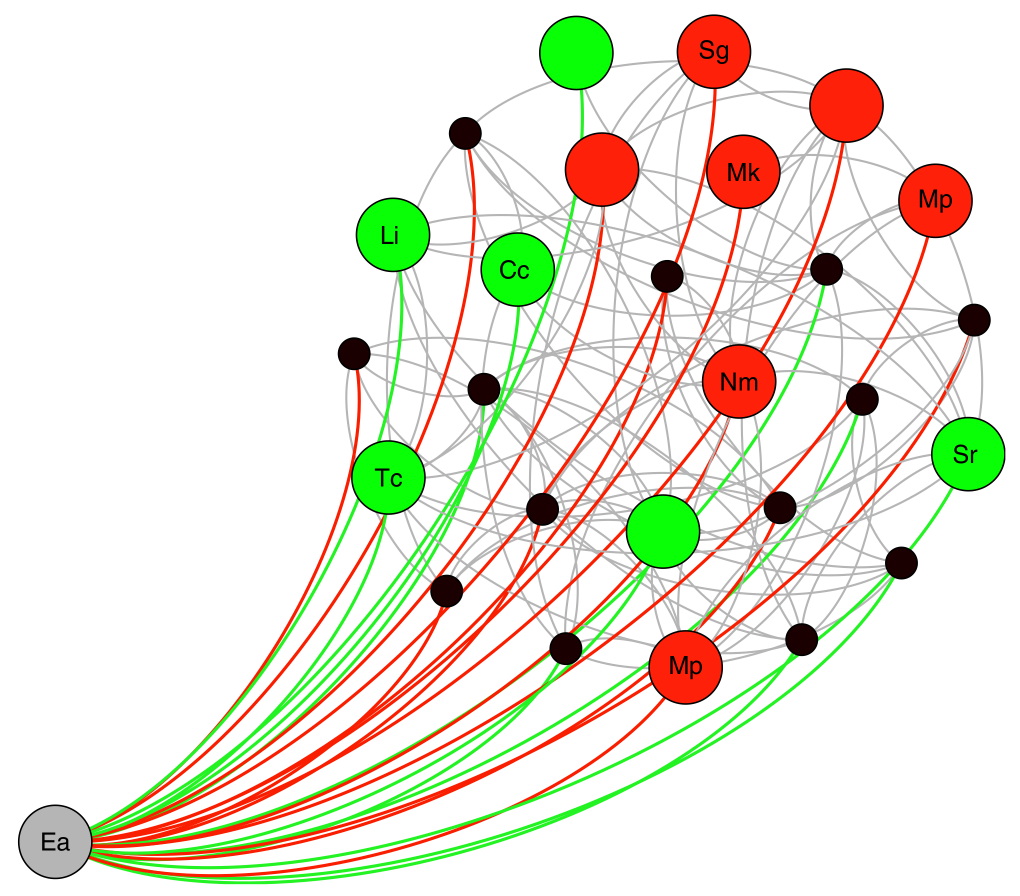
\includegraphics[width=.4\textwidth]{\fignet/JFS16-EnvirMicrobiol-Fig4} \\
    \refer{JFS16}
    \end{tabular}
  \end{tabular}
}

% %====================================================================
% \section*{'Observed' networks}
% \frame{\frametitle{What about 'observed networks'}
% 
%   \paragraph{Popular models:} Stochastic block-model (SBM) / Latent block-model (LBM) \\ ~
% 
%   \begin{tabular}{cc}
%     \begin{tabular}{p{.4\textwidth}}
%       \paragraph{Data:} 215 microbial OTUs (genus) $\times$ 26 samples (medias) 
%       \\ ~
%         
%       \paragraph{LBM:}  
%       co-clustering of OTUs and samples accounting for: \\
%       sampling effort, mean species abundance, over-dispersion
%       \\~
%         
%       \paragraph{Results:} 6 OTUs clusters $\times$ 12 sample clusters \\
%       $+$ interaction strength between clusters
%     \end{tabular}
%     & 
%     \hspace{-.05\textwidth} 
%     \begin{tabular}{p{.5\textwidth}}
%     \includegraphics[width=.45\textwidth]{../FIGURES/ASR18-Fig3} \\
%     \Refer{Aubert \& al., soumis}
%     \end{tabular}
%   \end{tabular}
% 
%   }

%====================================================================
\section*{'Observed' networks}
\frame{\frametitle{What about 'observed networks'}

  \paragraph{Popular models:} Stochastic block-model (SBM) / Latent block-model (LBM) 

  \bigskip \bigskip 
  \begin{tabular}{cc}
    \begin{tabular}{p{.4\textwidth}}
      \paragraph{Data:} 288 bacteria (OTUs) $\times$ 483 plants 
      \\ ~
        
      \paragraph{LBM:}  
      co-clustering of OTUs and plants accounting for: \\
      sampling effort, mean species abundance, over-dispersion
      \\~
        
      \paragraph{Results:} 10 bacteria clusters $\times$ 4 plant clusters \\
      $+$ interaction strength between clusters
    \end{tabular}
    & 
    \hspace{-.05\textwidth} 
    \begin{tabular}{p{.5\textwidth}}
    \includegraphics[width=.45\textwidth]{../FIGURES/ASR18-Fig2} \\
    \Refer{Aubert \& al., soumis}
    \end{tabular}
  \end{tabular}

  }

%====================================================================
\frame{ \frametitle{References}
  {\footnotesize
   %\tiny
   \bibliography{/home/robin/Biblio/BibGene}
%    \bibliographystyle{/home/robin/LATEX/Biblio/astats}
   \bibliographystyle{alpha}
  }
}

%====================================================================
%====================================================================
\end{document}
%====================================================================
%====================================================================
